\documentclass[a4paper, 12pt]{article}
\usepackage{header}

\begin{document}
\pagestyle{fancy}
\section{Лекция 02 от 12.09.2016 \\Признаки сравнения и другие признаки сходимости знакопостоянных рядов}

\subsection{О знакопостоянных рядах}

В рамках этой лекции будем рассматривать только ряды с неотрицательными членами!

Очевидно, что последовательность частичных сумм $\{S_n \}$ в таких рядах не убывает. Следовательно, существует $\lim\limits_{n\rightarrow \infty}S_n \in [0, +\infty]$.

\begin{Statement}[Критерий сходимости рядов с неотрицательными членами]
	Ряд $\sum\limits_{n=1}^{\infty} a_n$ сходится тогда и только тогда, когда последовательность его частичных сумм ограничена сверху.
\end{Statement}

Это позволяет сократить запись для таких рядов. Однако для рядов общего вида такая запись смысла не имеет, поскольку ряды могут не иметь даже бесконечного придела частичных сумм, то есть не иметь предела вообще (как например любимый нами ряд $1 - 1 + 1 - 1 + \ldots$)
\begin{Designation} Ряд сходится: $\sum\limits_{n=1}^{\infty} a_n < \infty$; ряд расходится: $\sum\limits_{n=1}^{\infty} a_n = \infty$.
\end{Designation}

\subsection{Признаки сравнения}

\begin{Test}[Первый признак сравнения]
	Пусть $\sum\limits_{n=1}^{\infty} a_n$ и $\sum\limits_{n=1}^{\infty} b_n$ --- два ряда с неотрицательными членами, и начиная с какого-то $N\in \N$ для всех $n > N$ имеет место неравенство $a_n \le b_n$. Тогда:
	\begin{enumerate}
	\item если $\sum\limits_{n=1}^{\infty} b_n < \infty$, то $\sum\limits_{n=1}^{\infty} a_n < \infty$;
	\item если $\sum\limits_{n=1}^{\infty} a_n = \infty$, то $\sum\limits_{n=1}^{\infty} b_n = \infty$.
	\end{enumerate}
\end{Test}

\begin{proof} Достаточно доказать для случая, когда $a_n \le b_n$ уже при $n \ge 1$ (убрав, <<начало>> ряда, сходимость мы не поменяем).
\begin{enumerate}
\item Рассмотрим частичные суммы рядов: $S^a_n = a_1 + a_2 + \ldots + a_n,\ S^b_n = b_1 + b_2 + \ldots + b_n.$
Так как ряд $\sum\limits_{n=1}^{\infty} b_n$ сходится, то $\lim\limits_{n\to\infty} S^b_n = C$ для некоторого $C$. Последовательность $S^b_n$ очевидно неубывающая, так что $S^b_n \le C$ для любого $n$. А значит, для всех $n$ верно, что
$$ 0 \le S^a_n = a_1 + a_2 + \ldots + a_n \le b_1 + b_2 + \ldots + b_n \le C.$$
Это показывает, что  $S^a_n$ монотонная ограниченная последовательность, а значит она обязательно имеет конечный предел. Так что ряд $\sum\limits_{n=1}^{\infty} a_n$  сходится.
	
\item Прямо следует из первого пункта.
\end{enumerate}
\end{proof}

\begin{Test}[Второй признак сравнения]
	Пусть $\sum\limits_{n=1}^{\infty} a_n$ и $\sum\limits_{n=1}^{\infty} b_n$ --- два ряда с положительными членами и $a_n \asymp b_n$ (то есть $\exists c, C> 0 $ такие, что начиная с некоторого индекса $N$, \\$c < \cfrac{a_n}{b_n}<C$). Тогда $\sum\limits_{n=1}^{\infty} a_n$ и $\sum\limits_{n=1}^{\infty} b_n$ сходятся или расходятся одновременно.
\end{Test}

\begin{proof}
	Прямо следует из предыдущего признака, так как $ cb_n \leqslant a_n\leqslant Cb_n$. 
\end{proof}
\begin{Comment}
	Если $a_n \sim b_n$ при $n \rightarrow \infty$, то $a_n \asymp b_n$.
\end{Comment}
\begin{Examples}[тривиальный]
	$\sum\limits_{n=1}^{\infty} \sin\frac{1}{n} \sim \sum\limits_{n=1}^{\infty} \frac{1}{n}$ --- расходится.
\end{Examples}

\begin{Test}[Третий признак сравнения]
	Пусть $\sum\limits_{n=1}^{\infty} a_n$ и $\sum\limits_{n=1}^{\infty} b_n$ --- два ряда с неотрицательными членами и начиная с некоторого номера $N\in\N$ для всех $n>N$ верно $\cfrac{a_{n+1}}{a_n} \leqslant \cfrac{b_{n+1}}{b_n}$ Тогда: \begin{enumerate}
		\item если $\sum\limits_{n=1}^{\infty} b_n < \infty$, то $\sum\limits_{n=1}^{\infty} a_n < \infty$;
		\item если $\sum\limits_{n=1}^{\infty} a_n = \infty$, то $\sum\limits_{n=1}^{\infty} b_n = \infty$. 
	\end{enumerate}
\end{Test}
\begin{proof}
	По сути говоря, данный признак сравнивает скорости роста, а в остальном это практически то же самое, что первый признак сравнения. Что ж, сведем его к нему.
	
	Достаточно считать, что $\frac{a_{n+1}}{a_n} \leqslant \frac{b_{n+1}}{b_n}$ уже при $n \ge 1$. Для любого натурального $k$ мы можем представить элементы $a_k$ и $b_k$ следующим образом:
	\begin{align*}
	a_k &= a_1 \frac{a_2}{a_1}\frac{a_3}{a_2} \ldots \frac{a_k}{a_{k-1}} \\
	b_k &= b_1 \frac{b_2}{b_1}\frac{b_3}{b_2} \ldots \frac{b_k}{b_{k-1}}
	\end{align*}
	Согласно условию, $\frac{a_{i}}{a_{i-1}} \le \frac{b_i}{b_{i-1}}$ при $1 \le i \le k$. Таким образом, мы почти получили, что $a_k \le \dfrac{a_1}{b_1}b_k$. Но мы не знаем, как соотносятся элементы $a_1$ и $b_1$. Что ж, избавимся от них, введя новый ряд:
	$$
	\sum\limits_{n=1}^{\infty} b'_n = \sum\limits_{n=1}^{\infty}\frac{a_1}{b_1}b_n.
	$$ 
	Для него будет выполняться неравенство $a_k \le b'_k$. Тем самым, мы свели задачу к первому признаку сравнения.
\end{proof}

\begin{Comment}
	Отметим, что для любого $q \in [0,1)$ ряд $\sum\limits_{n=1}^{\infty} q^n$ сходится. Действительно, $$\lim\limits_{N\rightarrow\infty} \sum\limits_{n=1}^{N} q^n=\lim\limits_{N\rightarrow\infty}\frac{q(q^N-1)}{q-1} = \frac{q}{1-q}.$$
\end{Comment}

\subsection{Прочие признаки}

\begin{Test}[Признак д'Аламбера]\
		\begin{enumerate}
		\item 	Пусть $\sum\limits_{n=1}^{\infty} a_n$ --- ряд с положительными членами, и существует такое $q \in [0, 1)$, что начиная с некоторого номера $N$ верно, что $\frac{a_{n+1}}{a_n} \leqslant q$. Тогда ряд $\sum\limits_{n=1}^{\infty} a_n$ сходится.
		\item Пусть $\sum\limits_{n=1}^{\infty} a_n$ --- ряд с положительными членами, и начиная с некоторого номера $N$ верно, что $\frac{a_{n+1}}{a_n} \geqslant~1$. Тогда $a_n \nrightarrow 0$ и ряд $\sum\limits_{n=1}^{\infty} a_n$ расходится.
	\end{enumerate}
\end{Test}

\begin{proof}
\ 
\begin{enumerate}
	\item 	Следует из третьего признака сравнения при $b_n = q^n$. 
	\item <<Тут и доказвать нечего>> \textcopyright\ лектор (\textit{прим. ред.:} утверждение очевидно из самой формулировки).
\end{enumerate}
\end{proof}

Однако чаще используется признак д'Аламбера в предельной форме.

\begin{Consequence}[Предельный признак д'Аламбера]
Пусть для ряда $\sum\limits_{n=1}^{\infty} a_n$ с положительными членами существует предел $\lim\limits_{n\rightarrow\infty} \frac{a_{n+1}}{a_n} = \alpha \in [0; +\infty]$. Тогда справедливы следующие утверждения:
\begin{enumerate}
	\item если $\alpha < 1$, то ряд $\sum\limits_{n=1}^{\infty} a_n$ сходится;
	\item если $\alpha > 1$, то ряд $\sum\limits_{n=1}^{\infty} a_n$ расходится;
	\item если $\alpha = 1$, то ряд $\sum\limits_{n=1}^{\infty} a_n$ может как сходиться, так и расходиться. 
\end{enumerate}
\end{Consequence}

\begin{proof}
	\ 
	\begin{enumerate}
		\item 	Если $\lim\limits_{n\rightarrow\infty} \frac{a_{n+1}}{a_n} = \alpha$ и $\alpha < 1$, то $\exists N \in \mathbb{N}$ такой, что при любом $n > N$ $\alpha-\eps<\frac{a_{n+1}}{a_n} < \alpha+\eps$, причём $\alpha+\eps <1$. А значит, ряд сходится по признаку д'Аламбера.
		\item Аналогично.
		\item Например, ряд $\sum\limits_{n=1}^{\infty} 1$ --- расходится, а ряд $\sum\limits_{n=1}^{\infty} \frac{1}{n^2}$ --- сходится. 

	\end{enumerate}
\end{proof}
Заметим, что признак д'Аламбера довольно грубый, то есть существует некоторая <<мертвая зона>> рядов, про сходимость которых он ничего не может сказать (например, про ряд  $\sum\limits_{n=1}^{\infty} \frac{1}{n}$).

\begin{Consequence}
	Если для ряда $\sum\limits_{n=1}^{\infty} a_n$ с положительными членами верно, что $\varlimsup\limits_{n\rarr \infty} \frac{a_{n+1}}{a_{n}} < 1$, то ряд сходится, а если $\varliminf\limits_{n \rarr \infty} \frac{a_{n+1}}{a_{n}} > 1$, то расходится.
\end{Consequence}

\begin{Test}[Радикальный признак Коши]\ 
Рассмотрим ряд $\sum\limits_{n=1}^{\infty} a_n$ с неотрицательными членами.
	\begin{enumerate}
		\item 	Пусть существует такое $q \in [0, 1)$, что начиная с некоторого номера $N$ верно, что $\sqrt[n]{{{a_n}}} \leqslant q$. Тогда ряд $\sum\limits_{n=1}^{\infty} a_n$ сходится.
		\item 	Пусть существует бесконечное множество индексов $n$, для которых верно, что  $\sqrt[n]{{{a_n}}} \geqslant~1$. Тогда $a_n \nrightarrow 0$ и ряд $\sum\limits_{n=1}^{\infty} a_n $ расходится.
	\end{enumerate}
\end{Test}

\begin{proof}
	\ 
	\begin{enumerate}
		\item 	Следует из первого признака сравнения при $b_n = q^n$. 
		\item Очевидно по определению расходимости ряда.
	\end{enumerate}
\end{proof}

Аналогично признаку д'Аламбера, можно сформулировать данный признак в предельной форме.
\begin{Consequence}[Радикальный признак Коши в предельной форме]
	Пусть для ряда	 $\sum\limits_{n=1}^{\infty} a_n$ с неотрицательными членами существует предел $\lim\limits_{n\rightarrow\infty} \sqrt[n]{a_n} = A$, где $A \in [0, \infty]$. Тогда:
	\begin{enumerate}
		\item если $A < 1$, то ряд $\sum\limits_{n=1}^{\infty} a_n$ сходится;
		\item если $A > 1$, то ряд $\sum\limits_{n=1}^{\infty} a_n$ расходится.
	\end{enumerate}
	Или, более общо:
	\begin{enumerate}
	\item если $\varlimsup\limits_{n\rarr \infty} \sqrt[n]{a_n} < 1$, то ряд $\sum\limits_{n=1}^{\infty} a_n$ сходится;
	\item если $\varlimsup\limits_{n\rarr \infty} \sqrt[n]{a_n} > 1$, то $a_n \nrightarrow 0$ и ряд $\sum\limits_{n=1}^{\infty} a_n$ расходится.
	\end{enumerate}
\end{Consequence}
Заметим, что так как тут используется только верхний предел, этот признак несколько удобней, чем предельный признак д'Аламбера.

\begin{Examples}
Рассмотрим следующий ряд:
$$
\sum\limits_{n=1}^{\infty} 2^{-n+(-1)^n} = \frac{1}{4} + \frac{1}{2} + \frac{1}{16} + \frac{1}{8} + \ldots 
$$
Как можно заметить, у соседних элементов ряда наблюдается то рост в 2 раза, то убывание в 8 раз, и предельный признак д'Аламбера ничего не может сказать про сходимость. Однако воспользуемся радикальным признаком Коши:
$$
\lim_{n\rarr \infty} \sqrt[n]{2^{-n + (-1)^n}} = \lim_{n\rarr \infty} 2^{-1 + \left(\frac{-1}{n}\right)^n} = \frac{1}{2}.
$$
Как мы видим, ряд сходится.
\end{Examples}

\begin{Task}
Есть ли обратный пример, когда радикальный признак Коши не помогает, в отличие от признака д'Аламбера?
\end{Task}

Для разных рядов может быть удобнее использовать разные признаки сходимости. Например, ряд $\sum\limits_{n=1}^{\infty} \dfrac{1}{n!}$ однозначно лучше исследовать с помощью признака д'Аламбера.

Мы всё ещё не научились выяснять сходимость рядов вида $\sum\limits_{n = 1}^{\infty}\cfrac{1}{n^\alpha}$. Итуиция подсказвает, что он сходится при $\alpha > 1$, как и интеграл. Сейчас мы в этом убедимся. В этом нам поможет следующая теорема.

\begin{Test}[Интегральный признак Коши--Маклорена]

Пусть $f(x) \geqslant 0$ --- невозрастающая на $[1, \infty)$ функция. Тогда $\sum\limits_{n=1}^{\infty}f(n)$ и $\int\limits_1^{\infty}f(x)dx$ сходятся или расходятся одновременно. Причем в случае сходимости
$$
\int\limits_{N+1}^{\infty}f(x)dx \leqslant r_N = f(N+1) + f(N+2) + \ldots \leqslant \int\limits_N^\infty f(x)dx.
$$
\end{Test}

\begin{proof}
Для удобства введем две вспомогательные функции: $f_S(x) = f(x-1)$ и $S(x) = f(\lfloor x \rfloor)$.

\begin{center}
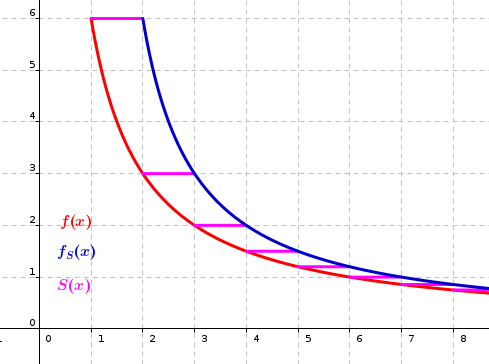
\includegraphics[scale=0.5]{03-01.png}
\end{center}

Тогда мы получаем, что $f(1) + f(2) + \ldots + f(N) = \int\limits_1^N S(x)dx$. Значит, ряд $\sum\limits_{n=1}^\infty f(n)$ сходится тогда и только тогда, когда сходится интеграл $\int\limits_1^\infty S(x)dx$. В свою очередь, несложно заметить, что сходимость этого интеграла влечет за собой сходимость интеграла $\int\limits^\infty_1 f(x)dx$, так как  при наших ограничениях $S(x) \geqslant f(x)$. С другой стороны, сходимость интеграла $\int\limits_1^\infty f(x)dx$ эквивалентна сходимости интеграла $\int\limits_2^\infty f_S(x)dx$, а она влечет за собой сходимость интеграла $\int\limits_1^\infty  S(x)dx$, так как $S(x) \leq f_S(x)$.

Отсюда же следует оценка для остатка. Действительно:
\begin{align*}
r_{N} = \int\limits_{N+1}^\infty S(x) dx & \leqslant \int_{N+1}^\infty f_S(x)dx = \int\limits_{N+1}^\infty f(x-1)dx = \int\limits_N^\infty f(x)dx, \\
r_{N} = \int\limits_{N+1}^\infty S(x)dx & \geqslant \int\limits_{N+1}^{\infty}f(x)dx.
\end{align*}
\end{proof}

\begin{Examples}
Допустим, мы хотим узнать сумму ряда $\sum\limits_{n=1}^{\infty}\frac{1}{n^3}$. Но поскольку ряд бесконечен, мы хотим обойтись первыми 100 членами, а чтобы оценить погрешность, посчитаем соответствующий интеграл.
$$
\int\limits_{n}^\infty \frac{1}{x^3} = -\frac{1}{2x^2} \Big|^\infty_{n} = \frac{1}{2n^2}
$$
Итого,
$$
\sum\limits_{n=1}^{\infty}\frac{1}{n^3} = \sum\limits_{n=1}^{100}\frac{1}{n^3} + \theta, \quad \text{где } \theta \in \left[\frac{1}{2\cdot101^2}, \frac{1}{2\cdot 100^2}\right].
$$

\end{Examples}

Подобным способом можно оценить асимптотику частичных сумм расходящегося ряда, например:
$$
\sum_{n=1}^{N} \frac{1}{\sqrt{n}} \sim 2\sqrt{n}
$$

Выводится это аналогично, просто теперь мы функциями $f(x)$, $f_S(x)$ и $S(x)$ оцениваем не остаток, а частичную сумму.

\end{document}
